\section{Příklad 3}
% Jako parametr zadejte skupinu (A-H)
\tretiZadani{H}

Metoda uzlových napětí využívá prvního Kirchhoffova zákona, který říká, že \textit{součet proudů vstupujících do uzlu se rovná součtu proudů z uzlu vystupujících}. V obvodu se libovolnému uzlu přiřadí nulový elektrický potenciál, poté se  označí napětí mezi tímto zvoleným \textit{referenčním uzlem} a všemi zbývajícími uzly, pro všechny uzly kromě referenčního se sestaví odpovídající rovnice podle prvního Kirchhoffova zákona, do které se dosadí proudy vyjádřené pomocí neznámých napětí mezi uzly a referenčním uzlem.

V zadaném obvodu máme označena uzlová napětí $U_A$, $U_B$, $U_C$, referenčním uzlem tak je uzel \textcolor{blue}{\textit{Ref}}, jak je naznačeno na obrázku \ref{fig:circ-3-1}. Na obrázku jsou také zaznačeny všechny proudy a napětí. Jejich orientace jsou zvoleny \uv{pocitově}, v případě, že by neodpovídaly skutečnému směru proudu v daném bodě, při výpočtech by pouze vyšly záporně. Důležité je používat směry všude stejně.
\begin{figure}[ht]
    \centering
    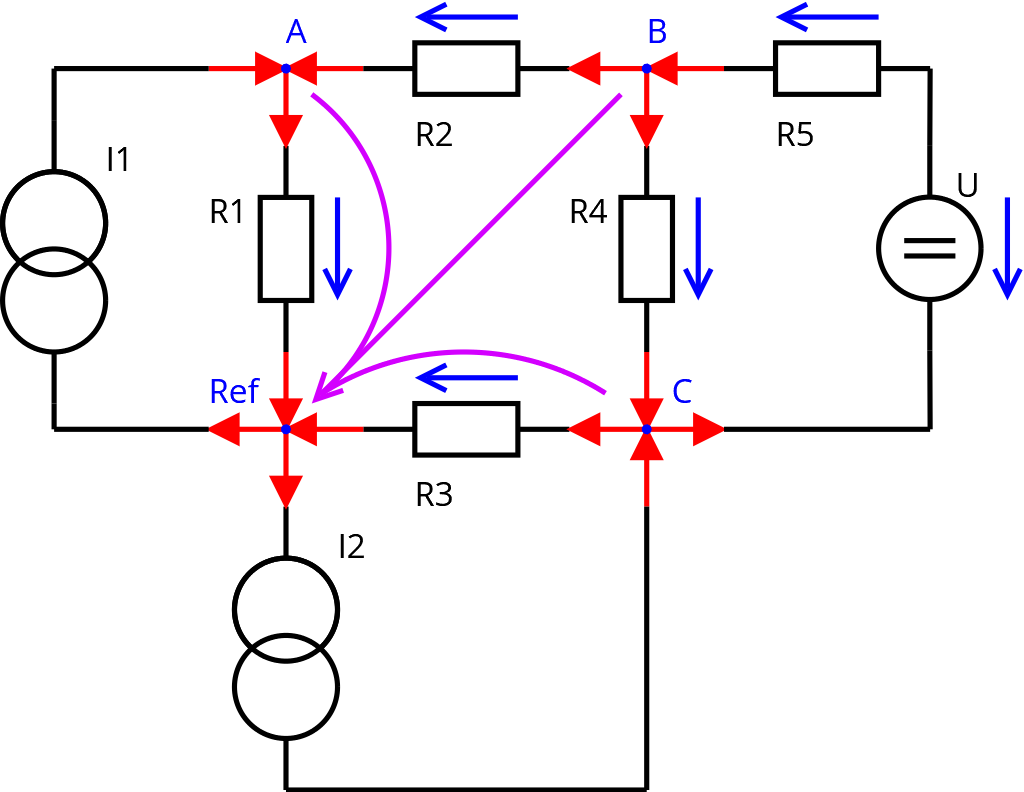
\includegraphics[width=10cm]{diagrams/Diagram10.png}
    \caption{Obvod s pojmenovanými uzly a zaznačenými směry proudů a napětí.}
    \label{fig:circ-3-1}
\end{figure}

Pro jednotlivé uzly můžeme nyní sestavit rovnice\footnote{Není nutné sestavovat rovnici pro referenční uzel. Kdybychom to udělali, při eliminaci matice této soustavy by vznikl nulový řádek, tato rovnice tak pro řešení soustavy nemá žádný vliv.}:
\begin{gather*}
    \textcolor{blue}{A}: I_1 + I_{R_2} - I_{R_1} = 0 \\
    \textcolor{blue}{B}: I_{R_5} - I_{R_2} - I_{R_4} = 0 \\
    \textcolor{blue}{C}: I_{R_4} - I_2 - I_{R_3} - I_{R_5} = 0 \\
\end{gather*}

Soustavu můžeme zapsat pomocí rozšířené matice, kde proměnnými jsou $I_{R_{1..5}}$, na pravou stranu přesuneme známé konstanty $I_1$ a $I_2$:
\begin{equation} \label{eq:circ-3-matrices}
\begin{pmatrix}[ccccc|c]
    -1 &  1 &  0 &  0 &  0 & -I_1 \\
     0 & -1 &  0 & -1 &  1 &  0 \\
     0 &  0 & -1 &  1 & -1 & -I_2
\end{pmatrix}
\sim
\begin{pmatrix}[ccccc|c]
     1 & -1 &  0 &  0 &  0 & I_1 \\
     0 &  1 &  1 &  0 &  0 & I_2 \\
     0 &  0 &  1 & -1 &  1 & I_2
\end{pmatrix}
\end{equation}
Vznikla soustava tří rovnic o pěti neznámých. Nyní musíme jednotlivé proudy vyjádřit pomocí uzlových napětí $U_A$, $U_B$ a $U_C$, měli bychom tak dostat soustavu tří rovnic se třemi neznámými, kterou můžeme vyřešit.

Proudy vyjádříme pomocí uzlových napětí, která přísluší daným odporům. Obvod si rozdělíme na~pomyslné \textit{náhradní obvody} pro jednotlivé proudy, jak je naznačeno na obrázku \ref{fig:circ-3-2}. V těchto náhradních obvodech pak s využitím Ohmova zákonu a druhého Kirchhoffova zákonu vyjádříme jednotlivé proudy:
\begin{equation}\label{eq:circ-3-currents}
\begin{gathered}
    -U_{R_1} + U_A = 0 \\
    -I_{R_1} R_1 = -U_A \\
    \mathbf{I_{R_1} = \frac{U_A}{R_1}} \\
    \\
    -U_{R_2} + U_B - U_A = 0 \\
    -I_{R_2} R_2 = -U_B + U_A \\
    \mathbf{I_{R_2} = \frac{U_B - U_A}{R_2}} \\
    \\
    -U_{R_3} + U_C = 0 \\
    -I_{R_3} R_3 = -U_C \\
    \mathbf{I_{R_3} = \frac{U_C}{R_3}} \\
    \\
    -U_{R_4} - U_C + U_B = 0 \\
    -I_{R_4} R_4 = -U_B + U_C \\
    \mathbf{I_{R_4} = \frac{U_B - U_C}{R_4}} \\
    \\
    U - I_{R_4} R_4 - I_{R_5} R_5 = 0 \\
    U - (U_B - U_C) - I_{R_5} R_5 = 0 \\
    \mathbf{I_{R_5} = \frac{U - U_B + U_C}{R_5}}
\end{gathered}
\end{equation}
\begin{figure}[ht]
    \centering
    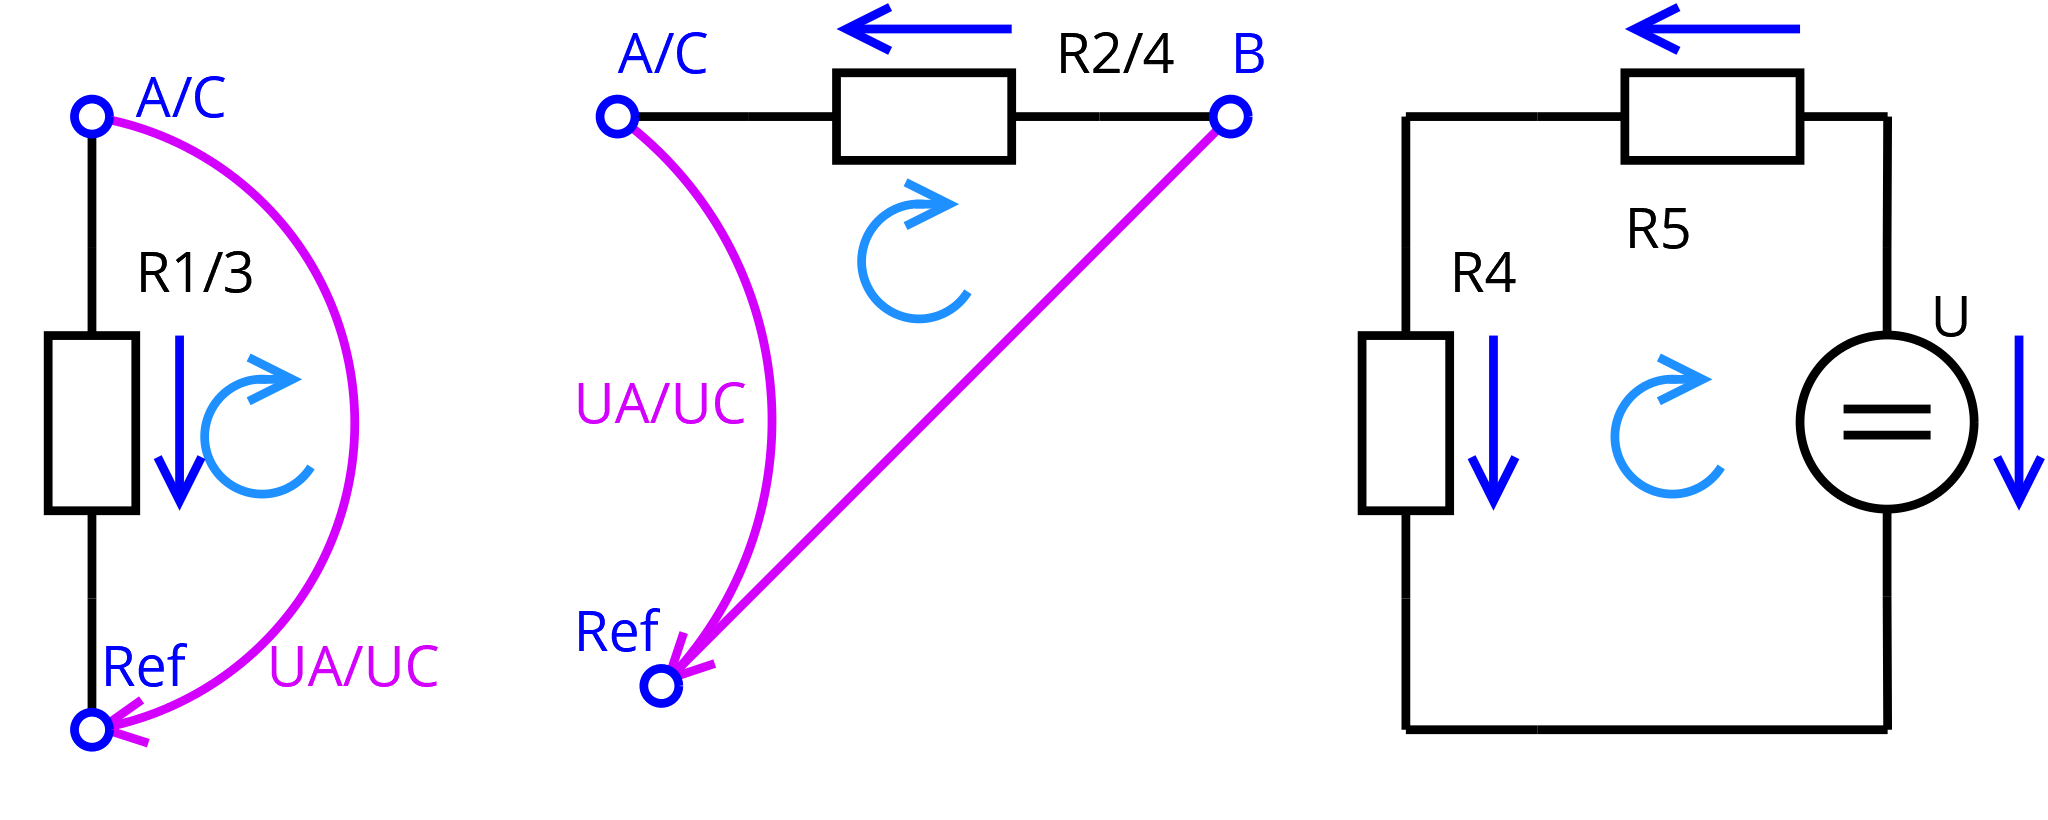
\includegraphics[width=14cm]{diagrams/Diagram11.png}
    \caption{Náhradní obvody pro jednotlivé proudy se smyčkami odpovídajícími vyjádření v \eqref{eq:circ-3-currents}. Obvody pro $R_1$ a $R_3$, resp. pro $R_2$ a $R_4$ jsou prakticky totožné, proto jsou schematicky zaznačeny najednou.}
    \label{fig:circ-3-2}
\end{figure}


Vyjádřené proudy nyní dosadíme do rovnic vytvořených podle matice \eqref{eq:circ-3-matrices} a výrazy upravíme do~podoby rovnice pro neznámé $U_A$, $U_B$, $U_C$:
\begin{gather*}
    \frac{U_A}{R_1} - \frac{U_B - U_A}{R_2} = I_1 \\
    U_A R_2 - U_B R_1 + U_A R_1 = I_1 R_1 R_2 \\
    (R_1 + R_2) U_A - R_1 U_B = I_1 R_1 R_2 \\
    \\
    \frac{U_B - U_A}{R_2} + \frac{U_C}{R_3} = I_2 \\
    - R_3 U_A + R_3 U_B + R_2 U_C = I_2 R_2 R_3 \\
    \\
    \frac{U_C}{R_3} + \frac{U_C - U_B}{R_4} + \frac{U - U_B + U_C}{R_5} = I_2 \\
    U_C R_4 R_5 + (U_C - U_B) R_3 R_5 + (U - U_B + U_C) R_3 R_4 = I_2 R_3 R_4 R_5 \\
    (-R_3 R_5 - R_3 R_4) U_B + (R_4 R_5 + R_3 R_5 + R_3 R_4) U_C = I_2 R_3 R_4 R_5 - U R_3 R_4
\end{gather*}
Pro přehlednost můžeme zapsat do matice pro neznámé $U_A$, $U_B$, $U_C$:
\begin{equation*}
\begin{pmatrix}[ccc|c]
R_1+R_2 & -R_1           &   0                     & I_1 R_1 R_2 \\
   -R_3 &  R_3           & R_2                     & I_2 R_2 R_3 \\
      0 & -R_3 (R_4+R_5) & R_3 (R_4+R_5) + R_4 R_5 & I_2 R_3 R_4 R_5-U R_3 R_4 
\end{pmatrix}
\end{equation*}
Nyní už můžeme dosadit hodnoty ze zadání a spočítat jednotlivá uzlová napětí:
\[
\begin{pmatrix}
 86 &   -47 &    0 \\
-58 &    58 &   39 \\
  0 & -3074 & 3774
\end{pmatrix}\begin{bmatrix}
U_A \\ U_B \\ U_C
\end{bmatrix} = \begin{bmatrix}
1741{,}35 \\ 1131 \\ -190\ 820
\end{bmatrix}
\]
\[
\begin{bmatrix}
U_A \\ U_B \\ U_C
\end{bmatrix} \approx \begin{bmatrix}
\num{60.504} \\ \num{73.6595} \\ \num{9.4354}
\end{bmatrix}
\]

Hledané hodnoty $I_{R_4}$ a $U_{R_4}$ nyní spočítáme velmi jednoduše dosazením do příslušné rovnice z \eqref{eq:circ-3-currents}:
\begin{gather*}
    I_{R_4} = \frac{U_B - U_C}{R_4} \\
    I_{R_4} = \frac{\num{73.6595}-\num{9.4354}}{28} \\
    \mathbf{I_{R_4} = \SI{2.2937}{\ampere}} \\
    \\
    U_{R_4} = R_4 I_{R_4} =  \frac{U_B - U_C}{R_4} R_4 = U_B - U_C \\
    U_{R_4} = \num{73.6595}-\num{9.4354} \\
    \mathbf{U_{R_4} = \SI{64.2241}{\volt}}
\end{gather*}
Obdobně bychom mohli snadno spočítat napětí a proud na jakémkoliv dalším rezistoru.
